\documentclass[12pt,dvipdfmx]{beamer}

\usepackage{graphicx}
\DeclareGraphicsExtensions{.pdf}
\DeclareGraphicsExtensions{.eps}
\graphicspath{{out/tex/svg/}{out/tex/lsvg/}{out/pdf/svg/}}
\usepackage{listings}
\usepackage{fancybox}
\usepackage{hyperref}
\usepackage{color}

\newcommand{\plusequal}{\mbox{\tt\ += }}
\newcommand{\minusequal}{\mbox{\tt\ -= }}
\newcommand{\divequal}{\mbox{\tt\ /= }}
\newcommand{\plusplus}{\mbox{\tt\ ++ }}



%% OpenMP section numbers
\newcommand{\sectionompparallel}{2.5}
\newcommand{\sectionompdeterminenumthreads}{2.5.1}
\newcommand{\sectionompfor}{2.7.1}
\newcommand{\sectionompdataenv}{2.14}
\newcommand{\sectionompgetnumthreads}{3.2.2}
\newcommand{\sectionompgetmaxthreads}{3.2.3}
\newcommand{\sectionompgetthreadnum}{3.2.4}


%%%%%%%%%%%%%%%%%%%%%%%%%%%
%%% themes
%%%%%%%%%%%%%%%%%%%%%%%%%%%
%\usetheme{Szeged} 
\usetheme{Madrid}

%% no navigation bar
% default boxes Bergen Boadilla Madrid Pittsburgh Rochester
%% tree-like navigation bar
% Antibes JuanLesPins Montpellier
%% toc sidebar
% Berkeley PaloAlto Goettingen Marburg Hannover Berlin Ilmenau Dresden Darmstadt Frankfurt Singapore Szeged
%% Section and Subsection Tables
% Copenhagen Luebeck Malmoe Warsaw

%%%%%%%%%%%%%%%%%%%%%%%%%%%
%%% innerthemes
%%%%%%%%%%%%%%%%%%%%%%%%%%%
% \useinnertheme{circles}       % default circles rectangles rounded inmargin

%%%%%%%%%%%%%%%%%%%%%%%%%%%
%%% outerthemes
%%%%%%%%%%%%%%%%%%%%%%%%%%%
% outertheme
% \useoutertheme{default}       % default infolines miniframes smoothbars sidebar sprit shadow tree smoothtree


%%%%%%%%%%%%%%%%%%%%%%%%%%%
%%% colorthemes
%%%%%%%%%%%%%%%%%%%%%%%%%%%
\usecolortheme{seahorse}
%% special purpose
% default structure sidebartab 
%% complete 
% albatross beetle crane dove fly seagull 
%% inner
% lily orchid rose
%% outer
% whale seahorse dolphin

%%%%%%%%%%%%%%%%%%%%%%%%%%%
%%% fontthemes
%%%%%%%%%%%%%%%%%%%%%%%%%%%
\usefonttheme{serif}  
% default professionalfonts serif structurebold structureitalicserif structuresmallcapsserif

%%%%%%%%%%%%%%%%%%%%%%%%%%%
%%% generally useful beamer settings
%%%%%%%%%%%%%%%%%%%%%%%%%%%
% 
\AtBeginDvi{\special{pdf:tounicode EUC-UCS2}}
% do not show navigation
\setbeamertemplate{navigation symbols}{}
% show page numbers
\setbeamertemplate{footline}[frame number]


%%%%%%%%%%%%%%%%%%%%%%%%%%%
%%% define some colors for convenience
%%%%%%%%%%%%%%%%%%%%%%%%%%%

%\newcommand{\mido}[1]{{\color{green}#1}}
\newcommand{\mido}[1]{{\color{green}#1}}
\newcommand{\mura}[1]{{\color{purple}#1}}
\newcommand{\ore}[1]{{\color{orange}#1}}
\newcommand{\ao}[1]{{\color{blue}#1}}
\newcommand{\aka}[1]{{\color{red}#1}}

\setbeamercolor{ex}{bg=cyan!20!white}

%%%%%%%%%%%%%%%%%%%%%%%%%%%
%%% how to typset code
%%%%%%%%%%%%%%%%%%%%%%%%%%%

\lstset{language = C,
numbers = left,
numberstyle = {\tiny \emph},
numbersep = 10pt,
breaklines = true,
breakindent = 40pt,
frame = tlRB,
frameround = ffft,
framesep = 3pt,
rulesep = 1pt,
rulecolor = {\color{blue}},
rulesepcolor = {\color{blue}},
flexiblecolumns = true,
keepspaces = true,
basicstyle = \ttfamily\scriptsize,
identifierstyle = ,
commentstyle = \it\scriptsize,
stringstyle = ,
showstringspaces = false,
tabsize = 4,
escapechar=\@,
}

\title{Analyzing Data Access of Algorithms 
  and How to Make Them Cache-Friendly?}
\institute{}
\author{Kenjiro Taura}
\date{}

\AtBeginSection[] % Do nothing for \section*
{
\begin{frame}
\frametitle{Contents}
\tableofcontents[currentsection]
\end{frame}
}

\AtBeginSubsection[] % Do nothing for \section*
{
\begin{frame}
\frametitle{Contents}
\tableofcontents[currentsection,currentsubsection]
\end{frame}
}

\begin{document}
\maketitle

%%%%%%%%%%%%%%%%%%%%%%%%%%%%%%%%%% 
\begin{frame}
\frametitle{Contents}
\tableofcontents
\end{frame}

%=================================
\section{Introduction}
%=================================

%%%%%%%%%%%%%%%%% 
\begin{frame}
\frametitle{Motivation}
\begin{itemize}
\item<1-> we've learned data access is an important factor 
  that determines performance of your program

\item<2-> it is thus clearly important to analyze how ``good''
  your algorithm is, in terms of data access
  performance

\item<3-> we routinely analyze computational
  complexity of algorithms to predict or explain
  algorithm performance, but it ignores the differing
  costs of accessing memory hierarchy (all memory accesses
  are $O(1)$)

\item<4-> we like to do 
  \ao{\em something analogous for data access}
\end{itemize}
\end{frame}

%=================================
\section{Analyzing data access complexity of serial programs}
%=================================

%=================================
\subsection{Overview}
%=================================

%%%%%%%%%%%%%%%%% 
\begin{frame}
\frametitle{Analyzing data access performance of serial programs}
\begin{columns}
\begin{column}{0.6\textwidth}
\begin{itemize}
\item<1-> we like to analyze data access cost of
  serial programs (on pencils and papers)

\item<2-> for this purpose, we calculate the amount of
  \ao{\em data transferred between levels of
    memory hierarchy}

\item<3-> in practical terms, this is a proxy of
  \ao{\em cache misses}

\item<4-> the analysis assumes a simple two level
  memory hierarchy
\end{itemize}
\end{column}

\begin{column}{0.4\textwidth}
\begin{center}
%\def\svgwidth{0.8\textwidth}
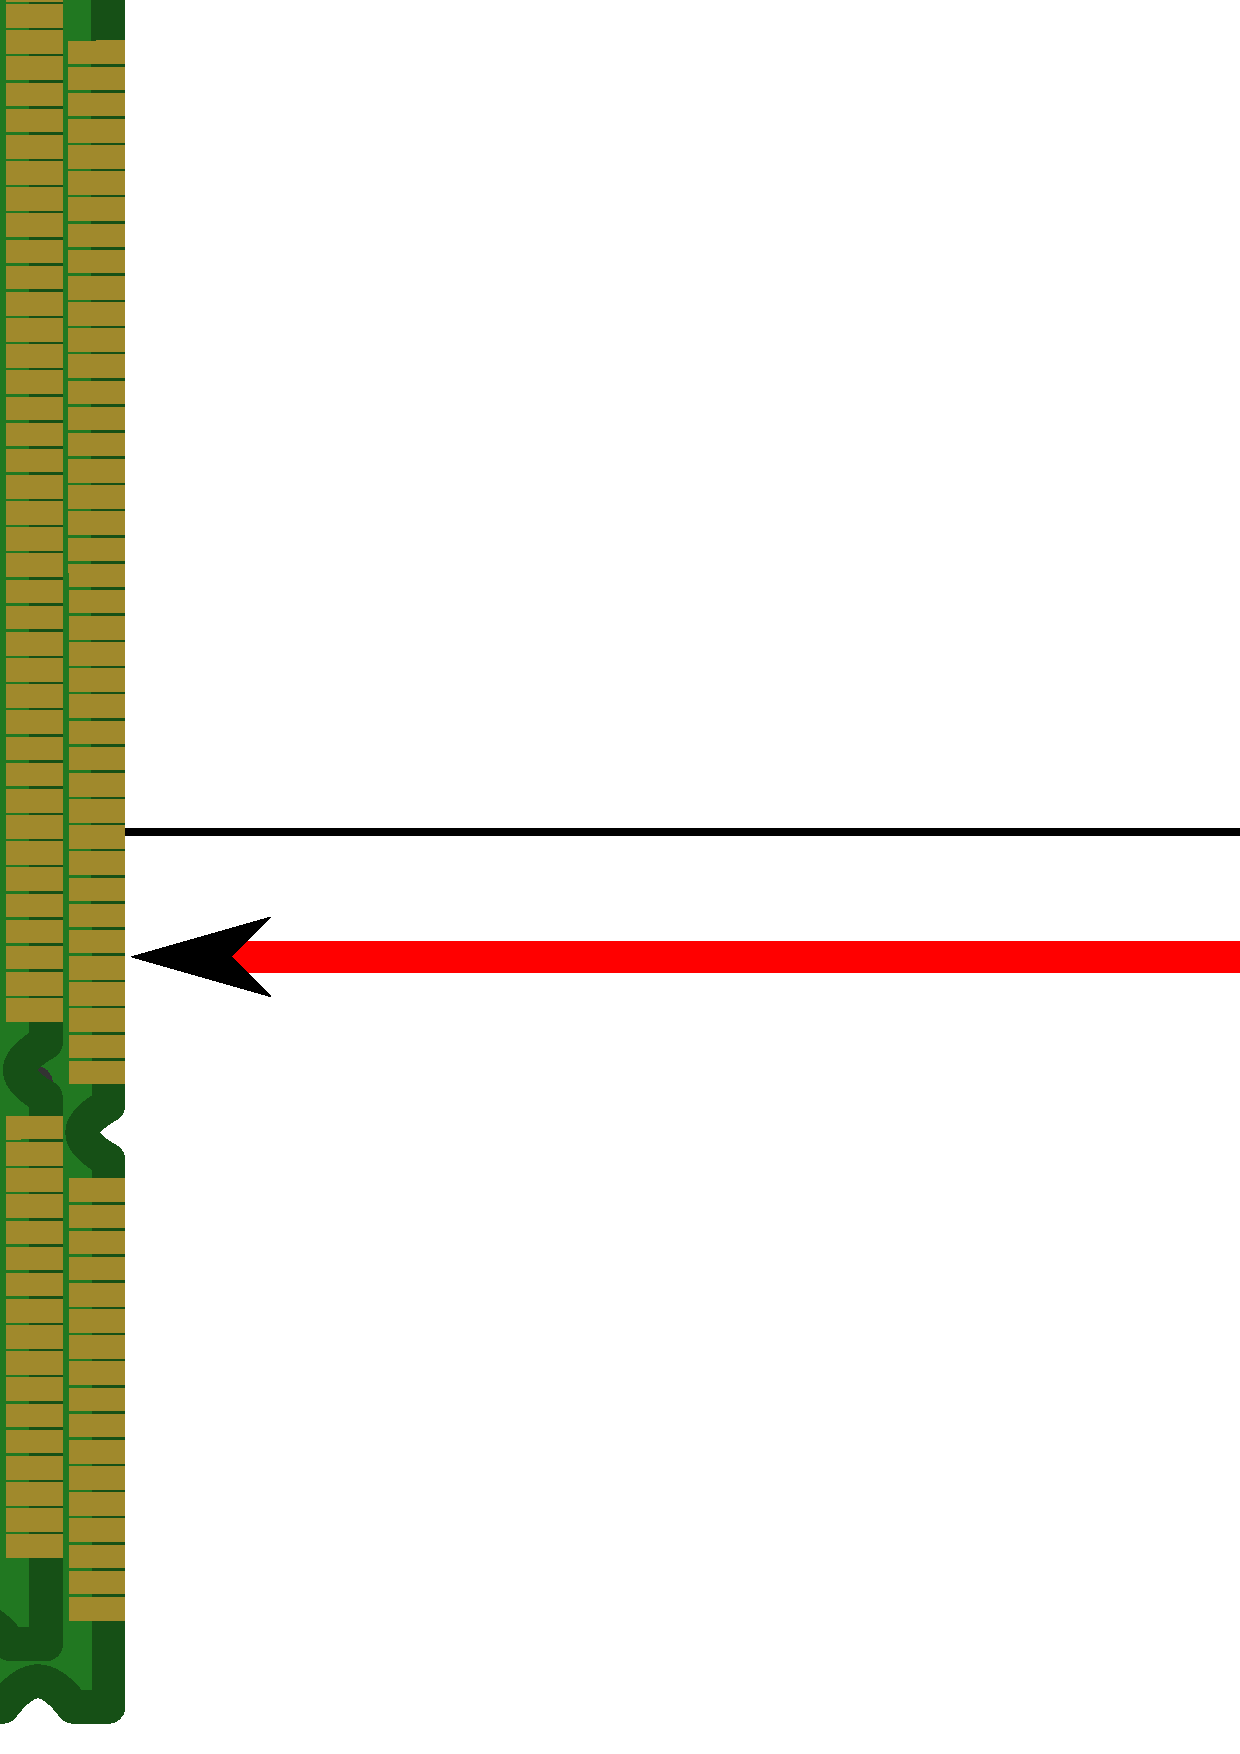
\includegraphics[width=0.8\textwidth]{out/pdf/svg/analysis_motivation.pdf}
\end{center}
\end{column}  
\end{columns}
\end{frame}

%=================================
\subsection{Model of a machine}
%=================================

%%%%%%%%%%%%%%%%% 
\begin{frame}
\frametitle{Model (of a single processor machine)}

\begin{columns}
\begin{column}{0.6\textwidth}
\begin{itemize}
\item<1-> a machine consists of 
  \begin{itemize}
  \item a processor,
  \item a fixed size cache ($C$ words), and
  \item an arbitrarily large main memory
  \item accessing a word not in the cache mandates 
    transferring the word into the cache
  \end{itemize}

\item<2-> the cache holds the most recently accessed
  $C$ words; $\approx$
  \begin{itemize}
  \item line size $=$ single word (whatever is convenient)
  \item fully associative
  \item LRU replacement
  \end{itemize}
\end{itemize}

\end{column}

\begin{column}{0.4\textwidth}
\begin{center}
\def\svgwidth{\textwidth}
{\scriptsize \input{out/tex/svg/cache_model.pdf_tex}}
\end{center}
\end{column}  
\end{columns}

\begin{center}
\aka{\em For now, we assume a single processor machine.}
\end{center}
\end{frame}

%%%%%%%%%%%%%%%%% 
\begin{frame}
\frametitle{Gaps between our model and real machines}
\begin{itemize}
\item<1-> \ao{hierarchical caches:}
\begin{columns}
  \begin{column}{0.6\textwidth}
    \begin{itemize}
    \item []
      $\Rightarrow$ each level can be easily modeled separately, with
      caches of various sizes
    \end{itemize}
  \end{column}
  \begin{column}{0.35\textwidth}
    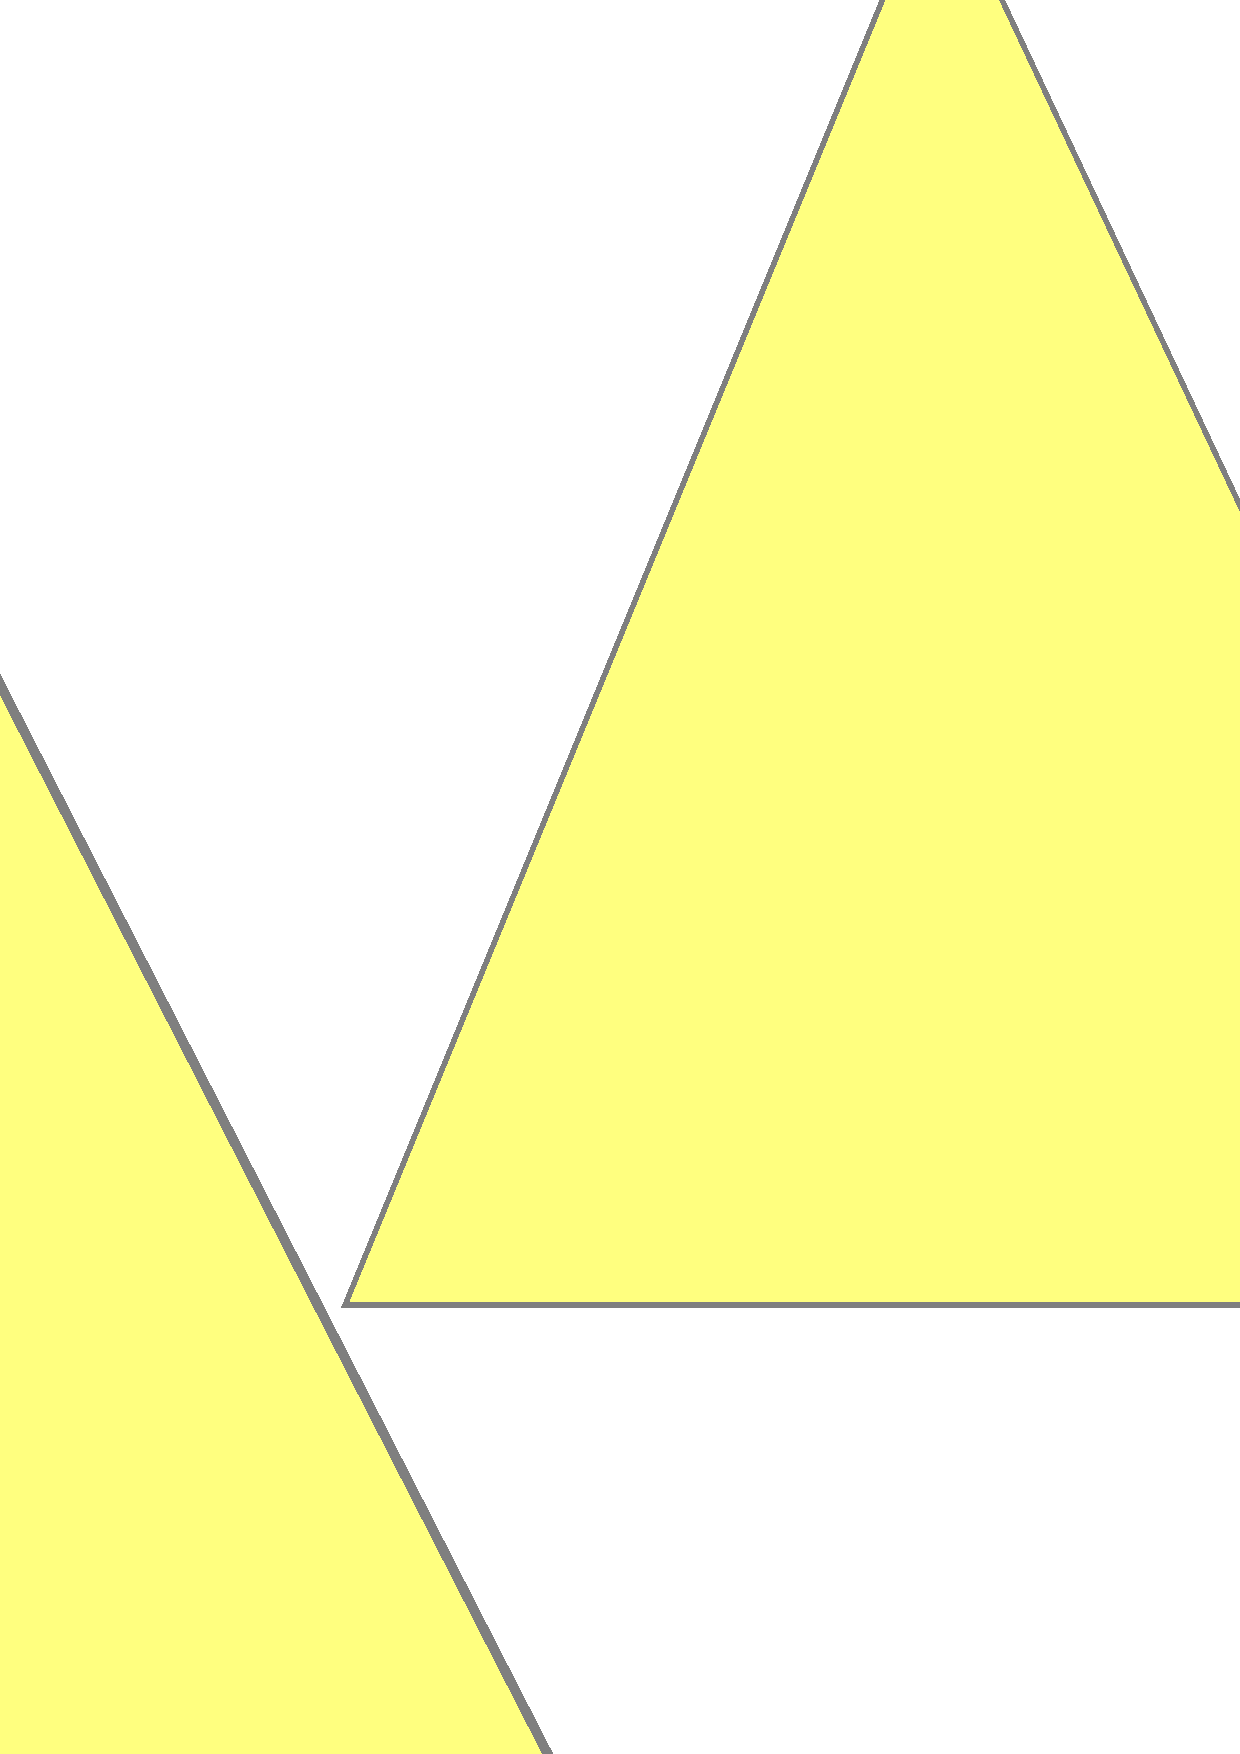
\includegraphics[width=0.8\textwidth]{out/pdf/svg/analysis_motivation_2.pdf}
  \end{column}
\end{columns}

\item<2-> \ao{concurrent accesses:}
  \begin{itemize}
  \item the model only counts the amount of data transferred
  \item in practice the cost heavily depends on how
    many concurrent accesses you have
  \item this model cannot capture the difference
    between link list traversal and random 
    array access
  \end{itemize}

\item<3-> \ao{prefetch:}
  \begin{itemize}
  \item similarly, this model 
    cannot capture the difference
    between sequential accesses that can take advantages of
    the hardware prefetcher and random accesses that cannot
  \end{itemize}
\end{itemize}
\end{frame}


%=================================
\subsection{An analysis methodology}
%=================================


%%%%%%%%%%%%%%%%% 
\begin{frame}
\frametitle{Terminologies}

\begin{itemize}
\item<1-> an \ao{\emph{execution}} of a program is the sequence of
  instructions 
\item<3-> an \ao{\emph{interval}} in an execution is a consecutive
  sequence of instructions in the execution
\item<4-> the \ao{\emph{working set}} of an interval is the
  number of \ao{\emph{distinct words}} accessed by the interval
\end{itemize}

\begin{center}
\only<1>{\def\svgwidth{0.8\textwidth}{\footnotesize\input{out/tex/svg/execution_interval_working_set_1.pdf_tex}}}%
\only<2>{\def\svgwidth{0.8\textwidth}{\footnotesize\input{out/tex/svg/execution_interval_working_set_2.pdf_tex}}}%
\only<3>{\def\svgwidth{0.8\textwidth}{\footnotesize\input{out/tex/svg/execution_interval_working_set_3.pdf_tex}}}%
\only<4>{\def\svgwidth{0.8\textwidth}{\footnotesize\input{out/tex/svg/execution_interval_working_set_4.pdf_tex}}}%
\end{center}
\end{frame}

%%%%%%%%%%%%%%%%% 
\begin{frame}
\frametitle{A basic methodology}
% \begin{columns}
% \begin{column}{0.6\textwidth}

\begin{itemize}
\item [] to calculate the amount of data 
  transferred in an execution,

  \begin{enumerate}
  \item<1-> split an execution into intervals each of which
    fits in the cache; i.e.,
    \[ \ao{\mbox{working set size of an interval } \leq C \mbox{ (cache size)}} \quad\quad (\ast) \]

  \item<2-> then, each interval transfers at most $C$ words, 
    because
    each word misses at most only once in the interval

  \item<3-> therefore,
    \[ 
    \ao{\mbox{data transferred} \leq \sum_{I : \mbox{all intervals}}
    \mbox{working set size of }I} \]
    \end{enumerate}
  \end{itemize}

% \end{column}
% \begin{column}{0.4\textwidth}
\begin{center}
\def\svgwidth{0.7\textwidth}
{\footnotesize\input{out/tex/svg/analyze_cache.pdf_tex}}
\end{center}
% \end{column}
% \end{columns}

\end{frame}


%%%%%%%%%%%%%%%%% 
\begin{frame}
\frametitle{Remarks}
\begin{itemize}
\item<1-> the condition ($\ast$) is important to bound 
  data transfers from above
  \[ \ao{\mbox{working set size of an interval } \leq C \mbox{ (cache size)}} \quad\quad (\ast) \]

\item<2-> each word in an interval misses at most only once, because
  \begin{itemize}
  \item the cache is LRU, and
  \item the condition ($\ast$) guarantees 
    that each word is never evicted within the interval
  \end{itemize}

\item<3-> in practical terms, an essential step to
  analyze data transfer is to \ao{\em identify the
    largest intervals that fits in the cache}
\end{itemize}
\end{frame}

%=================================
\section{Applying the methodology to matrix multiply}
%=================================

%%%%%%%%%%%%%%%%% 
\begin{frame}[fragile]
\frametitle{Applying the methodology}
\begin{itemize}

\item we will apply the methodology to some of the 
  algorithms we have studied so far

\item the key is to \ao{\em find subproblems (intervals) that fit in the cache}
\end{itemize}
\end{frame}


%%%%%%%%%%%%%%%%% 
\begin{frame}[fragile]
\frametitle{Analyzing the triply nested loop}
\begin{columns}[t]
\begin{column}{0.55\textwidth}
\begin{itemize}
\item []
\begin{lstlisting}
for (i = 0; i < n; i++) {
  for (j = 0; j < n; j++) {
    for (k = 0; k < n; k++) {
      C(i,j) += A(i,k) * B(k,j);
    }
  }
}
\end{lstlisting}
\item perform \ao{$n^3$} FMAs on \ao{$3n^2$} words
\item key question:
  \ao{\emph{which iteration fits in the cache?}}
\end{itemize}
\end{column}

\begin{column}{0.45\textwidth}
\begin{center}
\def\svgwidth{0.9\textwidth}
{\tiny \input{out/tex/svg/gemm_loop_1.pdf_tex}}
\end{center}
\end{column}
\end{columns}
\end{frame}


%%%%%%%%%%%%%%%%% 
\begin{frame}[fragile]
\frametitle{Working sets}
\begin{columns}

\begin{column}{0.5\textwidth}
\begin{lstlisting}
for (i = 0; i < n; i++) {
  for (j = 0; j < n; j++) {
    for (k = 0; k < n; k++) {
      C(i,j) += A(i,k) * B(k,j);
    }
  }
}
\end{lstlisting}

\begin{tabular}{|l|c|}\hline
level    & working set size  \\\hline
$I$ loop & $3n^2$            \\  
$J$ loop & $2n + n^2$        \\  
$K$ loop & $1 + 2n$          \\
$K$ iteration & $3$          \\\hline
\end{tabular}
\end{column}

\begin{column}{0.5\textwidth}
\begin{center}
\def\svgwidth{0.9\textwidth}
{\tiny \input{out/tex/svg/gemm_loop_1.pdf_tex}}
\end{center}
\end{column}
\end{columns}
\end{frame}

%%%%%%%%%%%%%%%%% 
\begin{frame}[fragile]
\frametitle{Cases to consider}
\begin{columns}
  \begin{column}{0.5\textwidth}
    \begin{itemize}
    \item<2-> Case 1: working set of \ao{the entire $I$-loop} fits in the cache ($3n^2 \leq C$)
    \item<3-> Case 2: working set of \ao{a single $I$-iteration ($=$ $J$-loop)} fits in the cache
      ($2n+n^2 \leq C$)
    \item<4-> Case 3: working set of \ao{a single $J$-iteration ($=$ $K$-loop)} fits in the cache
      ($1+2n \leq C$)
    \item<5-> Case 4: none of the above ($1+2n > C$)
    \end{itemize}
  \end{column}

  \begin{column}{0.5\textwidth}
    \begin{itemize}
    \item []
      \only<1>{\tiny\def\svgwidth{0.9\textwidth}\input{out/tex/svg/gemm_loop_1.pdf_tex}}%
      \only<2>{\tiny\def\svgwidth{0.9\textwidth}\input{out/tex/svg/gemm_loop_2.pdf_tex}}%
      \only<3>{\tiny\def\svgwidth{0.9\textwidth}\input{out/tex/svg/gemm_loop_3.pdf_tex}}%
      \only<4->{\tiny\def\svgwidth{0.9\textwidth}\input{out/tex/svg/gemm_loop_4.pdf_tex}}
    \end{itemize}
  \end{column}
\end{columns}

\begin{itemize}
  \item<6->[]
    Goal: for each case, bound $R(n)$ from the above,
    the traffic between memory and cache for $n \times n$ matrix-multiply
\end{itemize}

\end{frame}


%%%%%%%%%%%%%%%%% 
\begin{frame}[fragile]
\frametitle{Case 1 ($3n^2 \leq C$)}
\begin{columns}
  \begin{column}{0.5\textwidth}
\begin{itemize}
\item trivially, each element misses the cache only once. thus,
  \[ R(n) \leq 3n^2 = \ao{\frac{3}{n}} \cdot n^3 \]
\end{itemize}
\end{column}

\begin{column}{0.5\textwidth}
  \begin{itemize}
  \item []
{\tiny\def\svgwidth{0.9\textwidth}
\input{out/tex/svg/gemm_analyze_loop_case_1.pdf_tex}}
\end{itemize}
\end{column}
\end{columns}

\begin{itemize}
\item 
\ao{interpretation:} each element of $A$, $B$, and $C$ are reused $n$ times
\end{itemize}
\end{frame}


%%%%%%%%%%%%%%%%% 
\begin{frame}[fragile]
\frametitle{Case 2 ($2n + n^2 \leq C$)}
\begin{itemize}
\item the maximum number of $I$-iterations whose working set fit in the cache is:
\end{itemize}
\begin{columns}
  \begin{column}{0.5\textwidth}
\begin{itemize}
\item []      
\[ a \approx \frac{C - n^2}{2n} \]
\item in $a$ iterations, each element misses only once, so
\end{itemize}
\end{column}

\begin{column}{0.5\textwidth}
  \begin{itemize}
  \item []
{\tiny\def\svgwidth{0.9\textwidth}
\input{out/tex/svg/gemm_analyze_loop_case_2.pdf_tex}}
\end{itemize}
\end{column}
\end{columns}

\begin{itemize}
\item []
\[ R(n) \leq 
= \frac{n}{a} (n^2 + 2an)
= \ao{\left(\frac{1}{a}+\frac{2}{n}\right)} n^3
\]
\item
\ao{interpretation:} each element of $B$ is reused $a$ times in the cache;
each element in $A$ or $C$ $n$ times 
\end{itemize}
\end{frame}

%%%%%%%%%%%%%%%%% 
\begin{frame}[fragile]
\frametitle{A Remark}
\begin{itemize}
\item for a particular access pattern of the
  matrix multiplication,
  a better bound can be obtained
\end{itemize}
\begin{columns}
  \begin{column}{0.5\textwidth}
    \begin{itemize}
    \item as we know all elements of $B$ are accessed in the same order in
      each $I$-iteration,
      $B$ stays in the cache for any number of $a$ iterations
    \end{itemize}
\end{column}

\begin{column}{0.5\textwidth}
  \begin{itemize}
  \item []
{\tiny\def\svgwidth{0.9\textwidth}
\input{out/tex/svg/gemm_analyze_loop_case_2.pdf_tex}}
\end{itemize}
\end{column}
\end{columns}

\begin{itemize}
\item so, in this case too, each element misses only once throughout the entire computation
  \[ \therefore R(n) \leq 3n^2 = \frac{3}{n} \cdot n^3 \]
\item note that this analysis is specific to matrix-matrix multiplication
\end{itemize}

\end{frame}


%%%%%%%%%%%%%%%%% 
\begin{frame}
\frametitle{Case 3 ($1 + 2n \leq C$)}
\begin{columns}
  \begin{column}{0.5\textwidth}
\begin{itemize}
\item the maximum number of $j$-iterations
  that fit in the cache is:
\[ b \approx \frac{C - n}{n + 1} \]
\item in $b$ iterations, each element misses only once, so
\[ R(n) \leq \frac{n^2}{b} (n + b(n + 1))
= \ao{\left(\frac{1}{b} + 1 + \frac{1}{n} \right)} n^3
\]
\end{itemize}
  \end{column}

  \begin{column}{0.5\textwidth}
    \begin{itemize}
    \item []
{\tiny\def\svgwidth{0.9\textwidth}\input{out/tex/svg/gemm_analyze_loop_case_3.pdf_tex}}
\end{itemize}
\end{column}
\end{columns}

\begin{itemize}
\item []
\ao{interpretation:} each element in $B$ is never reused; 
each element in $A$ $b$ times; 
each clement in $C$ many ($\propto n$) times 
\end{itemize}
\end{frame}

%%%%%%%%%%%%%%%%% 
\begin{frame}
\frametitle{A Remark}
\begin{columns}
  \begin{column}{0.5\textwidth}
\begin{itemize}
\item a similar argument shows that an entire row of $A$ stays in the cache
  for any number of $b$ iterations
\item so each element misses only once in the entire $J$-loop (an iteration of the $I$-loop)
\end{itemize}
  \end{column}

  \begin{column}{0.5\textwidth}
    \begin{itemize}
    \item []
{\tiny\def\svgwidth{0.9\textwidth}\input{out/tex/svg/gemm_analyze_loop_case_3.pdf_tex}}
\end{itemize}
\end{column}
\end{columns}
  \[ \therefore R(n) \leq (2n + n^2) n = n^3 + 2n^2 \]
\end{frame}

%%%%%%%%%%%%%%%%% 
\begin{frame}
\frametitle{Case 4 ($1 + 2n > C$)}
\begin{columns}
  \begin{column}{0.5\textwidth}
\begin{itemize}
\item the maximum number of $K$-iterations
  that fit in the cache is:
\[ c \approx \frac{C - 1}{2} \]
\item in each $c$ iterations, each element misses only once, so
\[ R(n) \leq \frac{n^3}{c} (2c + 1)
= \ao{\left(2 + \frac{1}{c}\right)} n^3
\]
\end{itemize}
  \end{column}

  \begin{column}{0.5\textwidth}
    \begin{itemize}
    \item []
{\tiny\def\svgwidth{0.9\textwidth}\input{out/tex/svg/gemm_analyze_loop_case_4.pdf_tex}}
\end{itemize}
\end{column}
\end{columns}

\begin{itemize}
\item []
\ao{interpretation:} each element of $B$ or $A$ never reused; each element of $C$
reused $c$ times
\end{itemize}
\end{frame}

%%%%%%%%%%%%%%%%% 
\begin{frame}
\frametitle{A Remark}
\begin{columns}
  \begin{column}{0.5\textwidth}
\begin{itemize}
\item similarly, the element of $C$ stays in the cache for any number of
  $c$ iterations
\item so, each element misses only once in the entire $k$-loop (an iteration of the $j$-loop)
\[ R(n) \leq (2n + 1) n^2 = 2n^3 + n^2 \]
\end{itemize}
  \end{column}

  \begin{column}{0.5\textwidth}
    \begin{itemize}
    \item []
{\tiny\def\svgwidth{0.9\textwidth}\input{out/tex/svg/gemm_analyze_loop_case_4.pdf_tex}}
\end{itemize}
\end{column}
\end{columns}

\begin{itemize}
\item []
\ao{interpretation:} each element of $B$ or $A$ never reused; each element of $C$
reused $n$ times
\end{itemize}
\end{frame}



%%%%%%%%%%%%%%%%% 
%% \begin{frame}
%% \frametitle{Summary}
%% \begin{itemize}
%% \item summarize $R(n)/n^3$, words/FMA ($\propto$ BYTES/FLOPS),
%%   the number of misses per multiply-add ($0 \sim 3$)
%% \item []
%% \begin{center}
%% \begin{tabular}{|l|c|c|}\hline
%% condition         & $R(n)/n^3$                      & range      \\\hline
%% $3n^2 \leq C$     & $\frac{3}{n}$                   & $\sim 0$   \\
%% $2n + n^2 \leq C$ & $\frac{1}{a} + \frac{2}{n}$     & $0 \sim 1$ \\
%% $1 + 2n \leq C$   & $\frac{1}{b} + 1 + \frac{1}{n}$ & $1 \sim 2$ \\ 
%% $1 + 2n > C$      & $2 + \frac{1}{c}$               & $2 \sim 3$ \\\hline
%% \end{tabular}
%% \end{center}
%% \end{itemize}
%% \end{frame}

%%%%%%%%%%%%%%%%% 
\begin{frame}
\frametitle{Summary}
\begin{itemize}
\item $n^3 / R(n)$ or the number of FMAs per memory accesses (cache miss)
\item []
\begin{center}
\begin{tabular}{|l|c|c|}\hline
condition         & $R(n)$       & $n^3/R(n)$ \\\hline
$2n + n^2 \leq C$ & $3n^2$       & $n/3$ \\
$1 + 2n \leq C$   & $2n^2 + n^3$ & $\approx 1$ \\ 
$1 + 2n > C$      & $n^2 + 2n^3$ & $\approx 1/2$ \\\hline
\end{tabular}
\end{center}
\end{itemize}
\end{frame}

%%%%%%%%%%%%%%%%% 
\begin{frame}
\frametitle{Can we do better for large matrices?}
\begin{itemize}
\item so far, we've discussed the traffic of the straightforward triply-nested loop
\item its conclusion can be summarized as
\begin{itemize}
  \item if a single matrix is larger than $B$,
    access to $B$ almost induces a cache miss
\item can we do better for large matrices?    
\end{itemize}
\end{itemize}

\begin{center}
\begin{tabular}{|l|c|c|}\hline
condition         & $R(n)$       & $n^3/R(n)$ \\\hline
$2n + n^2 \leq C$ & $3n^2$       & $n/3$ \\
$1 + 2n \leq C$   & $2n^2 + n^3$ & $\approx 1$ \\ 
$1 + 2n > C$      & $n^2 + 2n^3$ & $\approx 1/2$ \\\hline
\end{tabular}
\end{center}
\end{frame}
  
%%%%%%%%%%%%%%%%% 
\begin{frame}
\frametitle{A general strategy}
\begin{itemize}
\item<1-> in general, the traffic increases when 
  \ao{\emph{the same amount of computation has a large working set}}
\item<2-> assuming the entire computaiton you want to perform is given/fixed,
  to reduce the traffic, you arrange \ao{\it order} subcomputations
  so that \ao{\emph{each subcomputation does a lot of computation
    on the same amount of data}}
\item<3-> the notion is so important that it is variously called
  \begin{itemize}
  \item \ao{compute/data ratio,}
  \item \ao{flops/byte,} 
  \item \ao{compute intensity,} or
  \item \ao{arithmetic intensity}
  \end{itemize}
\item<4-> the key is to identify the unit of computation (task) 
  whose compute intensity is high \ao{(compute-intensive task)}
\end{itemize}
\end{frame}


%%%%%%%%%%%%%%%%% 
%% \begin{frame}
%% \frametitle{The straightforward loop in light of compute intensity}

%% \begin{center}
%% \begin{tabular}{|l|c|c|c|}\hline
%% level         & flops  & working set size & ratio    \\\hline
%% $I$ loop      & $2n^3$ & $3n^2$           & $2/3n$   \\  
%% $J$ loop      & $2n^2$ & $2n + n^2$       & $\sim \aka{2}$ \\  
%% $K$ loop      & $2n$   & $1 + 2n$         & $\sim \aka{1}$ \\
%% $K$ iteration & 2      & $3$              & $\aka{2/3}$    \\\hline
%% \end{tabular}
%% \end{center}

%% \begin{itemize}
%% \item the outermost loop has an $O(n)$ compute intensity
%% \item yet each iteration of which has only an $O(1)$ compute intensity
%% \end{itemize}
%% \end{frame}

%%%%%%%%%%%%%%%%% 
\begin{frame}[fragile]
\frametitle{Cache blocking (tiling)}

\begin{itemize}
\item for matrix multiplication, let $l$ be the maximum number
that satisfies $2l + l^2\leq C$ (i.e., \ao{$l \approx \sqrt{C}$}) and form
a subcomputation that performs a $(l \times l)$ matrix multiplication

\item ignoring remainder iterations, it looks like:
\begin{columns}
\begin{column}{0.5\textwidth}
\begin{lstlisting}
l = @$\sqrt{C} - {\rm small\;constant}$@;
for (ii = 0; ii < n; ii += l)
 for (jj = 0; jj < n; jj += l)
  for (kk = 0; kk < n; kk += l)
   @\ao{\em /* block below misses each}@
   @\ao{\em    element at most once */}@
   @\ao{\tt for (i = ii; i < ii + l; i++)}@
    @\ao{\tt for (j = jj; j < jj + l; j++)}@
     @\ao{\tt for (k = kk; k < kk + l; k++)}@
       @\ao{\tt A(i,j) += B(i,k) * C(k,j);}@
\end{lstlisting}
\end{column}
\begin{column}{0.5\textwidth}
\def\svgwidth{1.0\textwidth}
{\tiny\input{out/tex/svg/gemm_analyze_loop_blocking.pdf_tex}}
\end{column}
\end{columns}
\end{itemize}
\end{frame}


%%%%%%%%%%%%%%%%% 
\begin{frame}[fragile]
  \frametitle{Cache blocking (tiling)}
\begin{columns}
\begin{column}{0.55\textwidth}
\begin{itemize}
\item<1-> each block:
  \begin{itemize}
  \item performs \ao{$l^3$} FMAs and
  \item touches \ao{$3l^2$} distinct words,
  \end{itemize}

\item<2-> so, the traffic of the entire computation

\[ \leq 3l^2 \cdot \left(\frac{n}{l}\right)^3 = \frac{3}{l}n^3 = \frac{3}{\sqrt{C}}n^3 \]

\end{itemize}
\end{column}

\begin{column}{0.45\textwidth}
\begin{lstlisting}
l = @$\sqrt{C} - {\rm small\;constant}$@;
for (ii = 0; ii < n; ii += l)
 for (jj = 0; jj < n; jj += l)
  for (kk = 0; kk < n; kk += l)
   @\ao{\em /* block below misses each}@
   @\ao{\em   element at most once */}@
   @\ao{\tt for (i = ii; i < ii + l; i++)}@
    @\ao{\tt for (j = jj; j < jj + l; j++)}@
     @\ao{\tt for (k = kk; k < kk + l; k++)}@
      @\ao{\tt A(i,j) += B(i,k) * C(k,j);}@
\end{lstlisting}
\end{column}
\end{columns}
\end{frame}

%%%%%%%%%%%%%%%%% 
%% \begin{frame}[fragile]
%% \frametitle{Effect of cache blocking}

%% \begin{center}
%% \begin{tabular}{|l|c|c|}\hline
%% condition         & $R(n)/n^3$                      & range      \\\hline
%% $3n^2 \leq C$     & ${\displaystyle\frac{3}{n}}$    & $\sim 0$   \\\hline
%% $2n + n^2 \leq C$ & ${\displaystyle\frac{1}{a} + \frac{2}{n}}$     & $0 \sim 1$ \\\hline
%% $1 + 2n \leq C$   & ${\displaystyle\frac{1}{b} + 1 + \frac{1}{n}}$ & $1 \sim 2$ \\ \hline
%% $1 + 2n > C$      & ${\displaystyle2 + \frac{1}{c}}$               & $2 \sim 3$ \\\hline
%% blocking          & \ao{${\displaystyle\frac{3\sqrt{3}}{\sqrt{C}}}$} & below \\\hline
%% \end{tabular}
%% \end{center}

%% \begin{itemize}
%% \item assume a word $=$ 4 bytes ({\tt float})
%% \begin{center}
%%   \begin{tabular}{|l|r|r|r|}\hline
%% bytes & $C$ & $l$ & $R(n)/n^3$ \\\hline
%% 32K   & 8K  & 52  & \ao{0.72}  \\
%% 256K  & 64K & 147 & \ao{0.43}  \\
%% 3MB   & 768K & 886 & \ao{0.0059} \\\hline
%% \end{tabular}
%% \end{center}
%% \end{itemize}
%% \end{frame}

%%%%%%%%%%%%%%%%% 
\begin{frame}[fragile]
\frametitle{Effect of cache blocking}

\begin{center}
\begin{tabular}{|l|c|c|}\hline
condition         & $R(n)$       & $n^3/R(n)$  \\\hline
$2n + n^2 \leq C$ & $3n^2$       & $n/3$       \\\hline
$1 + 2n \leq C$   & $2n^2 + n^3$ & $\sim 1$    \\ \hline
$1 + 2n > C$      & $n^2 + 2n^3$ & $\sim 1/2$   \\\hline
blocking          & ${\displaystyle \frac{3}{\sqrt{C}}} n^3$ & ${\displaystyle \frac{\sqrt{C}}{3}}$ \\\hline
\end{tabular}
\end{center}

\begin{itemize}
\item assume a word $=$ 4 bytes ({\tt float})
\begin{center}
  \begin{tabular}{|l|r|r|r|}\hline
bytes & $C$ & $l$ & $n^3/R(n)$ \\\hline
32K   & 8K  & $\approx$ 90.50  & \ao{30.16}  \\
256K  & 64K & $\approx$ 256 & \ao{85.33}  \\
3MB   & 768K & $\approx$ 886 & \ao{295.60} \\\hline
\end{tabular}
\end{center}
\end{itemize}
\end{frame}


%%%%%%%%%%%%%%%%% 
\begin{frame}
\frametitle{Recursive blocking}
\begin{itemize}
\item the tiling technique just mentioned needs to determine $l$ 
  for a particular size ($=$ level)
\item it may have to do this at all levels (12 deep nested loop)?
\item we also (for the sake of simplicity) assumed all matrices are square
\item for generality, portability, simplicity, \ao{recursive blocking} may apply
\end{itemize}

\end{frame}


%%%%%%%%%%%%%%%%% 
\begin{frame}[fragile]
\frametitle{Recursively blocked matrix multiply}
\begin{columns}[t]
\begin{column}{0.47\textwidth}

\begin{center}
\def\svgwidth{0.8\textwidth}
{\tiny\input{out/tex/svg/gemm_decomp_2.pdf_tex}}
\end{center}

\end{column}
\begin{column}{0.43\textwidth}
\begin{lstlisting}[basicstyle=\scriptsize]
gemm(@$A, B, C$@) {
  if (@$(M,N,K) = (1,1,1)$@) {
    @$c_{11} \plusequal a_{11} * b_{11};$@
  } else if (@$\max(M,N,K)=M$@) {
    @gemm($A_1, B, C_1$);@
    @gemm($A_2, B, C_2$);@
  } else if (@$\max(M,N,K)=N$@) {
    @gemm($A, B_1, C_1$);@
    @gemm($A, B_1, C_2$);@
  } else { /* @$\max(M,N,K)=K$@ */
    @gemm($A_1, B_1, C$);@
    @gemm($A_2, B_2, C$);@
  }
}
\end{lstlisting}
\end{column}
\end{columns}

\begin{itemize}
\item it divides flops into two 
\item it divides two of the three matrices, 
along \ao{\em the longest} axis
\end{itemize}

\end{frame}

%%%%%%%%%%%%%%%%% 
\begin{frame}
\frametitle{Settings}
\begin{itemize}
\item<1-> a single \ao{word} $=$ a single floating point number
\item<1-> cache size \ao{$= C$ words}
\item<2-> let \ao{$R(M, N, K)$} be
  the number of words transferred between cache and memory when
  multiplying $M\times K$ and $K\times N$ matrices
  (the cache is initially empty)
\item<3-> let \ao{$R(w)$} be the maximum number of words transferred for 
  any matrix multiply of up to $w$ words in total:
\[ R(w) \equiv \max_{MK+KN+MN\leq w} R(M,N,K) \]
we want to bound $R(w)$ from the above
\item<4-> to avoid making analysis tedious, assume all matrices are
  \ao{``nearly square''}
\[ \max(M,N,K) \leq 2 \min(M,N,K) \]
\end{itemize}
\end{frame}

%%%%%%%%%%%%%%%%% 
\begin{frame}
\frametitle{The largest subproblem that fits in the cache}
\begin{itemize}
\item the working set of {\tt gemm(A,B,C)} is $(MK+KN+MN)$ (words)
\item it fits in the cache if this is $\leq C$
\item thus we have:
  \[ \therefore \ao{R(w) \leq C \quad (w \leq C)} \]
\end{itemize}
\end{frame}

%%%%%%%%%%%%%%%%% 
\begin{frame}
\frametitle{Analyzing cases that do not fit in the cache}

\begin{columns}[t]
\begin{column}{0.6\textwidth}
\begin{itemize}
\item<1-> when $MK+KN+MN > C$, the interval doing
  {\tt gemm(A,B,C)} is two subintervals, 
  each of which does \texttt{gemm} for slightly smaller matrices

\item<2-> in the ``nearly square'' assumption, 
  the working set becomes $\leq 1/4$ when we divide 3
  times

\item<3-> to make math simpler, we take it that
  the working set becomes 
  ${\displaystyle \leq \frac{1}{\sqrt[3]{4}}} (= 2^{-2/3})$ of the
  original size on each recursion. i.e.,
\end{itemize}
\end{column}

\begin{column}{0.4\textwidth}
\begin{center}
\def\svgwidth{0.8\textwidth}
{\tiny \input{out/tex/svg/gemm_decomp_2.pdf_tex}}
\end{center}
\end{column}
\end{columns}

\only<4->{
\[ \therefore \ao{R(w) \leq 2 R(w / \sqrt[3]{4}) \quad (w > C)} \]
}
\end{frame}

%%%%%%%%%%%%%%%%% 
\begin{frame}
\frametitle{Combined}
\begin{itemize}
\item we have:
\begin{equation*}
R(w) \leq \left\{
\begin{array}{ll}
w                   & (w \leq C) \\
2R(w / \sqrt[3]{4}) & (w > C) \\
\end{array}
\right.  
\end{equation*}

\item when $w > C$, it takes up to 
$d \approx \log_{\sqrt[3]{4}}(w/C)$
recursion steps until the working set becomes $\leq C$

\item the whole computation is essentially $2^d$
  consecutive intervals, each transferring $\leq C$ words
\end{itemize}
\end{frame}

%%%%%%%%%%%%%%%%% 
\begin{frame}
\frametitle{Illustration}
\begin{center}
\def\svgwidth{0.9\textwidth}
{\tiny\input{out/tex/svg/gemm_analyze_miss.pdf_tex}}
\end{center}

\begin{eqnarray*}
\therefore R(w) & < & 2^d \cdot C  \\
                & =  & 2^{\log_{\sqrt[3]{4}}(w/C)} \cdot C \\
                & =  & C \left(\frac{w}{C}\right)^{\frac{1}{\log\sqrt[3]{4}}} \\
                & = & \frac{1}{\sqrt{C}} w^{3/2}
\end{eqnarray*}
              
\end{frame}


%%%%%%%%%%%%%%%%% 
\begin{frame}
\frametitle{Result}
\begin{itemize}
\item we have:
\begin{equation*}
R(w) \leq \frac{1}{\sqrt{C}} w^{3/2}
\end{equation*}

\item for square $(n \times n)$ matrices ($w = 3n^2$),
\begin{equation*}
\therefore R(n) = R(3n^2) = \ao{\frac{3\sqrt{3}}{\sqrt{C}} n^3}
\end{equation*}

\item the same as the blocking we have seen before (not surprising), but
  we achieved this for all cache levels
  \end{itemize}
\end{frame}

%%%%%%%%%%%%%%%%% 
\begin{frame}[fragile]
\frametitle{A practical remark}

\begin{columns}[t]
\begin{column}{0.45\textwidth}
\begin{itemize}
\item<1-> in practice we stop recursion when the 
  matrices become ``small enough''

\item<2-> but how small is small enough? 

\item<3-> when the threshold $\leq$ level $x$ cache,
  the analysis holds for all levels $x$ and lower
\end{itemize}
\end{column}

\begin{column}{0.55\textwidth}
  \begin{itemize}
  \item []
\begin{lstlisting}[basicstyle=\scriptsize]
gemm(@$A, B, C$@) {
  if (@\aka{$A, B, C$ together fit in the cache}@) {
    @\aka{\tt for $(i,j,k) \in [0..M]\times[0..N]\times[0..K]$}@
      @\aka{$c_{ij} \plusequal a_{ik} * b_{kj};$}@
  } else if (@$\max(M,N,K)=M$@) {
    @gemm($A_1, B, C_1$);@
    @gemm($A_2, B, C_2$);@
  } else if (@$\max(M,N,K)=N$@) {
    @gemm($A, B_1, C_1$);@
    @gemm($A, B_1, C_2$);@
  } else { /* @$\max(M,N,K)=K$@ */
    @gemm($A_1, B_1, C$);@
    @gemm($A_2, B_2, C$);@
  }
}
\end{lstlisting}
  \end{itemize}
\end{column}
\end{columns}

\begin{itemize}
\item<4-> on the other hand, we like to make it large, 
  to reduce control overhead
\end{itemize}
\end{frame}

\iffalse
%%%%%%%%%%%%%%%%% 
\begin{frame}
\frametitle{Summary of the traffics}
\begin{itemize}
\item compare the recursive algorithm and the loop algorithm with the worst algorithm,
  which transfers three elements at every multiply-add ($R(n)n^3 = 3$)
\item $R(n)/n^3$ for algorithms we've seen so far:

\begin{center}
{\small
\begin{tabular}{|l|c|c|c|}\hline
          & case 2                & case 3               & case 4 \\
          & {\scriptsize $n(n+2) \leq C$} & {\scriptsize $2n+1 \leq C$} & {\scriptsize $2n+1 > C$} \\\hline
worst     & 3                     & 3                     &  3 \\\hline
loop      & $\ao{\displaystyle\frac{1}{a} + \frac{4}{n}}$ & ${\displaystyle 2 + \frac{1}{b} + \frac{2}{n}}$ & 3 \\\hline
recursive & ${\displaystyle\frac{6\sqrt{3}}{\sqrt{C}}}$ & ${\displaystyle\frac{6\sqrt{3}}{\sqrt{C}}}$ & ${\displaystyle\frac{6\sqrt{3}}{\sqrt{C}}}$ \\\hline
\end{tabular}}
\end{center}

\item it's clear the loop version does not accomplish much for case 3 and 4
\item let's look at the case 2: $\ao{\displaystyle\left(\frac{1}{a} + \frac{4}{n}\right)}$ a little deeper
\end{itemize}
\end{frame}
\fi


\iffalse
%%%%%%%%%%%%%%%%%
\section{Tools to measure cache/memory traffic}
%%%%%%%%%%%%%%%%% 

%%%%%%%%%%%%%%%%% 
\begin{frame}[fragile]
\frametitle{Tools to measure cache/memory traffic}
\begin{itemize}
\item analyzing data access performance is harder than
  analyzing computational efficiency (ignoring caches)
  \begin{itemize}
  \item the code reflects how much computation you do
  \item you can experimentally confirm your understanding
    by counting cycles (or wall-clock time)
  \end{itemize}

\item caches are complex and subtle
  \begin{itemize}
  \item the same data access expression (e.g., {\tt a[i]})
    may or may not count as the traffic
  \item gaps are larger between our model and the real machines
    (associativity, prefetches, local variables and stacks we
    often ignore, etc.)
  \end{itemize}

\item we like to have a tool to measure what
  happened on the machine $\rightarrow$ performance counters
\end{itemize}
\end{frame}


%%%%%%%%%%%%%%%%% 
\begin{frame}[fragile]
\frametitle{Performance counters}
\begin{itemize}
\item recent CPUs equip with \ao{\em performance counters},
  which count the number of times various events happen
  in the processor

\item OS exposes it to users (e.g., Linux 
  {\tt perf\_event\_open} system call)

\item there are tools to access them more conveniently 
  \begin{itemize}
  \item command: Linux perf ({\tt man perf})
  \item library: PAPI \url{http://icl.cs.utk.edu/papi/} 
  \item GUI: hpctoolkit \url{http://hpctoolkit.org/}, VTunes, \ldots
  \end{itemize}
\end{itemize}
\end{frame}

%=================================
\subsection{{\tt perf} command}
%=================================
%%%%%%%%%%%%%%%%% 
\begin{frame}[fragile]
\frametitle{{\tt perf} command}
\begin{itemize}
\item {\tt perf} command is particularly easy to use
\begin{lstlisting}
@\ao{\tt perf stat} {\it command line}@
\end{lstlisting}
will show you cycles, instructions, and some other info

\item to access performance counters of your interest (e.g., cache misses),
  specify them with \ao{\tt -e}
\begin{lstlisting}
perf stat @\ao{\tt -e {\it counter} -e {\it counter} \ldots}@  @{\it command line}@

\end{lstlisting}
\item to know the list of available counters
\begin{lstlisting}
@\ao{\tt perf list}@
\end{lstlisting}
\end{itemize}
\end{frame}


%%%%%%%%%%%%%%%%% 
\begin{frame}[fragile]
\frametitle{{\tt perf} command}
% \begin{columns}
% \begin{column}{0.6\textwidth}

\begin{center}
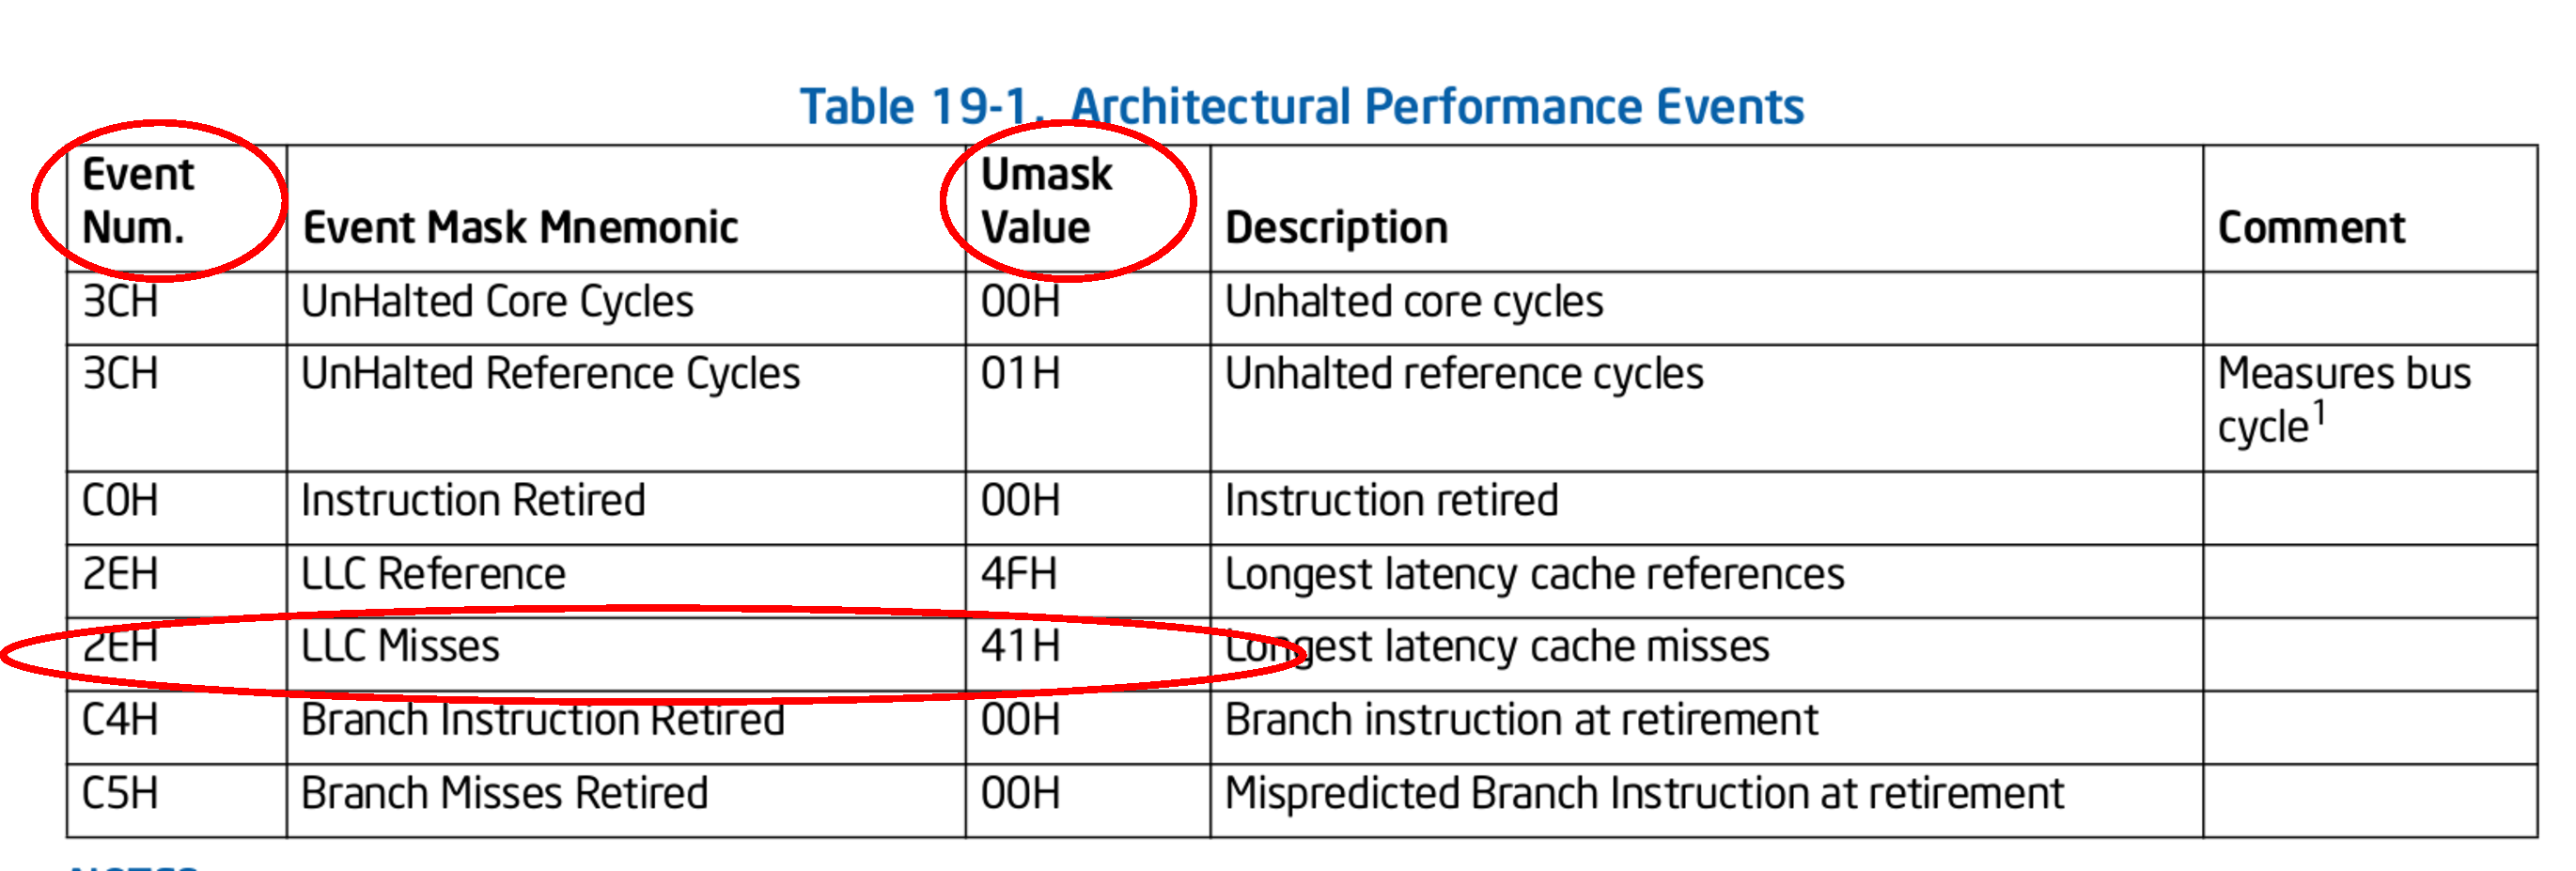
\includegraphics[width=0.6\textwidth]{out/pdf/svg/counters_table.pdf}
\end{center}
\begin{itemize}
\item many interesting counters are not listed by {\tt perf list}
\item we often need to resort to ``raw'' events 
  (defined on each CPU model)
\item consult intel document
\footnote{{\scriptsize Intel 64 and IA-32 Architectures Developer's Manual: 
Volume 3B: System Programming Guide, Part 2. Chapter 19 ``Performance Monitoring Events'' 
\url{http://www.intel.com/content/www/us/en/architecture-and-technology/64-ia-32-architectures-software-developer-vol-3b-part-2-manual.html}}}
\item if the table says Event Num $=$ {\tt 2EH}, Umask Value $=$ {\tt 41H}, then you can access it via perf by {\tt -e r412e} (umask; event num)
\end{itemize}
\end{frame}

%=================================
\subsection{PAPI library}
%=================================
%%%%%%%%%%%%%%%%% 
\begin{frame}
\frametitle{PAPI library}
\begin{itemize}
\item library for accessing performance counters
\item \url{http://icl.cs.utk.edu/papi/index.html}
\item basic concepts
  \begin{itemize}
  \item create an empty ``event set''
  \item add events of interest to the event set
  \item start counting
  \item do whatever you want to measure
  \item stop counting
  \end{itemize}
\item visit \url{http://icl.cs.utk.edu/papi/docs/index.html}
  and see ``Low Level Functions''
\end{itemize}
\end{frame}


%%%%%%%%%%%%%%%%% 
\begin{frame}[fragile]
\frametitle{PAPI minimum example (single thread)}
\begin{itemize}
\item A minimum example with a single thread and no error checks
\begin{lstlisting}
#include <papi.h>
int main() {






  @\mura{\{ do\_whatever(); \}}@


  return 0;
}
\end{lstlisting}
\end{itemize}
\end{frame}


%%%%%%%%%%%%%%%%% 
\begin{frame}[fragile]
\frametitle{PAPI minimum example (single thread)}
\begin{itemize}
\item A minimum example with a single thread and no error checks
\begin{lstlisting}
#include <papi.h>
int main() {
  @\ao{\tt PAPI\_library\_init}@(PAPI_VER_CURRENT);
  int es = PAPI_NULL; 
  @\ao{\tt PAPI\_create\_eventset}@(&es);
  @\ao{\tt PAPI\_add\_named\_event}@(es, "ix86arch::LLC_MISSES");
  @\ao{\tt PAPI\_start}@(es);
  long long values[1];
  @\mura{\{ do\_whatever(); \}}@
  @\ao{\tt PAPI\_stop}@(es, values);
  printf("%lld\n", values[0]);
  return 0;
}
\end{lstlisting}
\end{itemize}
\end{frame}

%%%%%%%%%%%%%%%%% 
\begin{frame}[fragile]
\frametitle{Compiling and running PAPI programs}
\begin{itemize}
\item compile and run
\begin{lstlisting}
$ gcc ex.c -lpapi
$ ./a.out
33
\end{lstlisting} %$
\item {\tt papi\_avail} and {\tt papi\_native\_avail} list
available event names (to pass to {\tt PAPI\_add\_named\_event})
\begin{itemize}
\item {\tt perf\_raw::r{\it nnnn}} for raw counters (same as perf command)
\end{itemize}
\end{itemize}
\end{frame}

%%%%%%%%%%%%%%%%% 
\begin{frame}[fragile]
\frametitle{Error checks}
\begin{itemize}
\item be prepared to handle errors 
  (never assume you know what works)!
\item many routines return {\tt PAPI\_OK} on success
  and a return code on error, which can then be passed
  to \ao{\tt PAPI\_strerror({\it return\_code})} to 
  convert it into an error message
\item encapsulate such function calls with this
\begin{lstlisting}
void check_(int ret, const char * fun) {
  if (ret != PAPI_OK) {
    fprintf(stderr, "%s failed (%s)\n", fun, @\ao{\tt PAPI\_strerror(ret)}@);
    exit(1);
  }
}

#define check(call) check_(call, #call)
\end{lstlisting}
\end{itemize}
\end{frame}


%%%%%%%%%%%%%%%%% 
\begin{frame}[fragile]
\frametitle{A complete example with error checks}
\begin{itemize}
\item []
\begin{lstlisting}[basicstyle = \ttfamily\tiny]
#include <stdio.h>
#include <stdlib.h>
#include <papi.h>

void check_(int ret, const char * fun) {
  if (ret != PAPI_OK) {
    fprintf(stderr, "%s failed (%s)\n", fun, @\ao{\tt PAPI\_strerror(ret)}@);
    exit(1);
  }
}
#define check(f) check_(f, #f)

int main() {
  int ver = PAPI_library_init(PAPI_VER_CURRENT);
  if (ver != PAPI_VER_CURRENT) {
    fprintf(stderr, "PAPI_library_init(%d) failed (returned %d)\n",
            PAPI_VER_CURRENT, ver);
    exit(1);
  }
  int es = PAPI_NULL;
  check(PAPI_create_eventset(&es));
  check(PAPI_add_named_event(es, "ix86arch::LLC_MISSES"));
  check(PAPI_start(es));
  @\mura{\{ do\_whatever(); \}}@
  long long values[1];
  check(PAPI_stop(es, values));
  printf("%lld\n", values[0]);
  return 0;
}
\end{lstlisting}
\end{itemize}
\end{frame}

%%%%%%%%%%%%%%%%% 
\begin{frame}
\frametitle{Multithreaded programs}
\begin{itemize}
\item must call \ao{\tt PAPI\_thread\_init({\it id\_fun})} in addition to
  {\tt PAPI\_library\_init(PAPI\_VER\_CURRENT)}
  \begin{itemize}
  \item {\it id\_fun} is a function that returns identity of a thread
    (e.g., {\tt pthread\_self, omp\_get\_thread\_num})
  \end{itemize}
\item each thread must call \ao{\tt PAPI\_register\_thread}
\item event set is private to a thread (each thread must call
  \ao{\tt PAPI\_create\_eventset(), PAPI\_start(), PAPI\_stop()})
\end{itemize}
\end{frame}

%%%%%%%%%%%%%%%%% 
\begin{frame}[fragile]
\frametitle{Multithreaded example}
\begin{itemize}
\item []
\begin{lstlisting}
#include <stdio.h>
#include <stdlib.h>
#include <omp.h>
#include <papi.h>
/* @{\tt check\_}@ and @{\tt check}@ omitted (same as single thread) */
int main() {
  /* error check for PAPI_library_init omitted (same as single thread) */
  PAPI_library_init(PAPI_VER_CURRENT);
  check(@\ao{\tt PAPI\_thread\_init}@((unsigned long(*)()) omp_get_thread_num));
#pragma omp parallel
  {
    check(@\ao{\tt PAPI\_register\_thread}@()); /* each thread must do this */
    int es = PAPI_NULL;
    check(PAPI_create_eventset(&es)); /* @\ao{\it each thread must create its own set}@ */
    check(PAPI_add_named_event(es, "ix86arch::LLC_MISSES"));
    check(PAPI_start(es));
    @\mura{\{ do\_whatever(); \}}@
    long long values[1];
    check(PAPI_stop(es, values));
    printf("thread %d: %lld\n", omp_get_thread_num(), values[0]);
  }
  return 0;
}
\end{lstlisting}
\end{itemize}
\end{frame}

%%%%%%%%%%%%%%%%% 
\begin{frame}
\frametitle{Several ways to obtain counter values}
\begin{itemize}
\item \ao{\tt PAPI\_stop({\it es}, {\it values})}: get current values and stop counting
\item \ao{\tt PAPI\_read({\it es}, {\it values})}: get current values and continue counting
\item \ao{\tt PAPI\_accum({\it es}, {\it values})}: accumulate current values, 
  reset counters, and continue counting
\end{itemize}
\end{frame}

%%%%%%%%%%%%%%%%% 
\begin{frame}
\frametitle{Useful PAPI commands}
\begin{itemize}
\item \ao{\tt papi\_avail, papi\_native\_avail}: list event counter names
\item \ao{\tt papi\_mem\_info}: report information about caches and TLB
(size, line size, associativity, etc.)
\end{itemize}
\end{frame}
\fi

%=================================
\iffalse
\section{Matching the model and measurements}
%=================================
%%%%%%%%%%%%%%%%% 
\begin{frame}
\frametitle{Matching the model and measurements (measurements)}
\begin{itemize}
\item \aka{warnings:}
  \begin{itemize}
  \item counters are highly CPU model-specific
  \item do not expect portability too much; always check
    {\tt perf list}, {\tt perf\_native\_avail}, and
    the Intel manual
  \item some counters or combination thereof
    cannot be monitored even if listed in {\tt
      perf\_native\_avail} (you fail to add it to
    event set; never forget to check return code)
  \item virtualized environments have none
    or limited support of performance counters;
    \aka{\em Amazon EC2 environment shows no counters
    available {\tt (; ;)}} (I don't know if there is a workaround)
  \end{itemize}

\item the following experiments were conducted
  on my Haswell (Core i7-4500U) laptop
  \begin{itemize}
  \item L1 : 32KB, L2 : 256KB, L3 : 4MB
  \end{itemize}
\end{itemize}
\end{frame}

%%%%%%%%%%%%%%%%% 
\begin{frame}
\frametitle{Matching the model and measurements (measurements)}
\begin{itemize}
\item relevant counters
  \begin{itemize}
  \item {\tt L1D:REPLACEMENT}
  \item {\tt L2\_TRANS:L2\_FILL}
  \item {\tt MEM\_LOAD\_UOPS\_RETIRED:L3\_MISS}
  \end{itemize}

\item cache miss counts do not include line transfers 
  hit thanks to prefetches
\item {\tt L1D:REPLACEMENT} and {\tt L2\_TRANS:L2\_FILL} 
  seem closer to what we want to match our model against
\item I could not find good counters for L3 caches, so 
  measure {\tt ix86arch::LLC\_MISSES}
\end{itemize}
\end{frame}

%%%%%%%%%%%%%%%%% 
\begin{frame}
\frametitle{Matching the model and measurements}
\begin{itemize}
\item counters give the number of \ao{\emph{cache lines}}
transferred
\item a line is 64 bytes and a word is 4 bytes, so we assume:

\ao{\emph{words}} transferred
$\approx 16 \times$ cache lines transferred

\item recall we have:
\[ R(w) \leq \frac{1}{\sqrt{C}} w^{3/2} \]
and $R(w)$ is the number of \ao{\emph{words}} transferred

\item so we calculate:
\[ \frac{\mbox{the number of cache lines transferred}}{w^{3/2}} \]
(and expect it to be close to ${\displaystyle{\frac{1}{\sqrt{C}}}}$
for $w > C$)

\end{itemize}
\end{frame}

%%%%%%%%%%%%%%%%% 
\begin{frame}
\frametitle{${\displaystyle{1/\sqrt{C}}}$}
\begin{center}
\begin{tabular}{|l|c|c|}\hline
level & $C$ & $\frac{1}{\sqrt{C}}$ \\\hline
L1    & 8K  & $0.011048\cdots$ \\
L2    & 64K & $0.003906\cdots$ \\
L3    & 1M  & $0.000976\cdots$ \\\hline
\end{tabular}
\end{center}
\end{frame}

%%%%%%%%%%%%%%%%% 
\begin{frame}
\frametitle{L1 (recursive blocking)}
\begin{center}
\def\svgwidth{0.8\textwidth}  
%{\footnotesize\input{out/tex/data/mm/mm_blocking_l1rep_10000}}
out/tex/data/mm/mm\_blocking\_l1rep\_10000
\end{center}

\begin{itemize}
\item they are not constant as we expected
\end{itemize}
\end{frame}

%%%%%%%%%%%%%%%%% 
\begin{frame}
\frametitle{What are the spikes?}
\begin{itemize}
\item it spikes when $M = $ a large power of two 
  ($128 | M$, to be more specific)
\item analyzing why it's happening is a good exercise for you
\item whatever it is, I told you avoid it!
\item let's remove $M$'s that are multiple of 128
\end{itemize}
\end{frame}

%%%%%%%%%%%%%%%%% 
\begin{frame}
\frametitle{L1 (remove multiples of 128)}
\begin{columns}
  \begin{column}{0.7\textwidth}
\begin{center}
\def\svgwidth{0.8\textwidth}  
%{\footnotesize\input{out/tex/data/mm/mm_blocking_l1rep_128}}
out/tex/data/mm/mm\_blocking\_l1rep\_128
\end{center}
  \end{column}
  \begin{column}{0.3\textwidth}
    \begin{tabular}{|c|c|}\hline
 $M$  & value  \\\hline
 1808 & 0.0187 \\
 1856 & 0.0178 \\
 1872 & 0.0177 \\
 1936 & 0.0170 \\
 1984 & 0.0159 \\
 2000 & 0.0167 \\\hline
    \end{tabular}
\[ \frac{1}{\sqrt{C}} \approx 0.011048\cdots \]
  \end{column}
\end{columns}
\end{frame}

%%%%%%%%%%%%%%%%% 
\begin{frame}
\frametitle{L1 (compare w/ and w/o recursive blocking)}
\begin{center}
\def\svgwidth{0.8\textwidth}  
%{\footnotesize\input{out/tex/data/mm/mm_compare_l1rep_128}}
out/tex/data/mm/mm\_compare\_l1rep\_128
\end{center}
\end{frame}

%%%%%%%%%%%%%%%%% 
\begin{frame}
\frametitle{L1 (remove multiples of 64)}
\begin{center}
\def\svgwidth{0.8\textwidth}  
%{\footnotesize\input{out/tex/data/mm/mm_compare_l1rep_64}}
out/tex/data/mm/mm\_compare\_l1rep\_64
\end{center}
\end{frame}

%%%%%%%%%%%%%%%%% 
\begin{frame}
\frametitle{L1 (remove multiples of 32)}
\begin{center}
\def\svgwidth{0.8\textwidth}  
%{\footnotesize\input{out/tex/data/mm/mm_compare_l1rep_32}}
out/tex/data/mm/mm\_compare\_l1rep\_32
\end{center}
\end{frame}

%%%%%%%%%%%%%%%%% 
\begin{frame}
\frametitle{L2}
\begin{center}
\def\svgwidth{0.8\textwidth}  
%{\footnotesize\input{out/tex/data/mm/mm_blocking_l2fill_10000}}
out/tex/data/mm/mm\_blocking\_l2fill\_10000
\end{center}
\end{frame}

%%%%%%%%%%%%%%%%% 
\begin{frame}
\frametitle{L2 (remove multiples of 128)}
\begin{columns}
  \begin{column}{0.7\textwidth}
\begin{center}
\def\svgwidth{0.8\textwidth}  
%{\footnotesize\input{out/tex/data/mm/mm_blocking_l2fill_128}}
out/tex/data/mm/mm\_blocking\_l2fill\_128
\end{center}
  \end{column}
  \begin{column}{0.3\textwidth}
    \begin{tabular}{|c|c|}\hline
 $M$  & value  \\\hline
 1808 & 0.00499 \\
 1856 & 0.00481 \\
 1872 & 0.00511 \\
 1936 & 0.00470 \\
 1984 & 0.00476 \\
 2000 & 0.00505 \\\hline
    \end{tabular}
\[ \frac{1}{\sqrt{C}} \approx 0.003906\cdots \]
  \end{column}  
\end{columns}

\end{frame}

%%%%%%%%%%%%%%%%% 
\begin{frame}
\frametitle{L2 (compare w/ and w/o recursive blocking)}
\begin{center}
\def\svgwidth{0.8\textwidth}  
%{\footnotesize\input{out/tex/data/mm/mm_compare_l2fill_128}}
out/tex/data/mm/mm\_compare\_l2fill\_128
\end{center}
\end{frame}

%%%%%%%%%%%%%%%%% 
\begin{frame}
\frametitle{L2 (no multiples of 64)}
\begin{center}
\def\svgwidth{0.8\textwidth}  
%{\footnotesize\input{out/tex/data/mm/mm_compare_l2fill_64}}
out/tex/data/mm/mm\_compare\_l2fill\_64
\end{center}
\end{frame}


%%%%%%%%%%%%%%%%% 
\begin{frame}
\frametitle{L2 (no multiples of 32)}
\begin{center}
\def\svgwidth{0.8\textwidth}  
%{\footnotesize\input{out/tex/data/mm/mm_compare_l2fill_32}}
out/tex/data/mm/mm\_compare\_l2fill\_32
\end{center}
\end{frame}


\fi                             %end of section{matching the model and measurements}

%=================================
\section{Analyzing merge sort}
%=================================
%%%%%%%%%%%%%%%%% 
\begin{frame}[fragile]
\frametitle{Review: (serial) merge sort}
\begin{columns}
\begin{column}{0.45\textwidth}
\begin{lstlisting}
/* sort a..a_end and put the result into
   (i)  a (if dest = 0)
   (ii) t (if dest = 1) */
void @\ao{\tt ms}@(elem * a, elem * a_end, 
        elem * t, int dest) {
  long n = a_end - a;
  if (n == 1) {
    if (dest) t[0] = a[0];
  } else {
    /* split the array into two */
    long nh = n / 2;
    elem * c = a + nh;
    /* sort 1st half */
    @\ao{\tt ms}@(a, c,     t,      1 - dest);
    /* sort 2nd half */
    @\ao{\tt ms}@(c, a_end, t + nh, 1 - dest);
    elem * s = (dest ? a : t);
    elem * d = (dest ? t : a);
    /* merge them */
    @\mura{\tt merge}@(s,      s + nh, 
          s + nh, s + n, d);
  }
}
\end{lstlisting}
\end{column}

\begin{column}{0.43\textwidth}
\begin{lstlisting}
/* merge a_beg ... a_end 
     and b_beg ... b_end 
    into c */
void 
@\mura{merge}@(elem * a, elem * a_end, 
      elem * b, elem * b_end, 
      elem * c) {
  elem * p = a, * q = b, * r = c;
  while (p < a_end && q < b_end) {
    if (*p < *q) { *r++ = *p++; }
    else { *r++ = *q++; }
  }
  while (p < a_end) *r++ = *p++;
  while (q < b_end) *r++ = *q++;
}
\end{lstlisting}

\aka{note:} as always, actually switch to serial sort below a threshold
  (not shown in the code above)
\end{column}
\end{columns}
\end{frame}

%%%%%%%%%%%%%%%%% 
\begin{frame}[fragile]
\frametitle{Memory $\leftrightarrow$ cache transfer in merge sort (1)
\\ base case}
\begin{itemize}
\item merge sorting $n$ elements takes \ao{\em two}
  arrays of $n$ elements each, and touch all elements of them
  \ao{\em $\Rightarrow$ the working set is $2n$ words}

\item thus, it fits in the cache when $2n \leq C$
\[ \therefore \ao{R(n) \leq 2n \quad (2n \leq C)} \]
\end{itemize}
\end{frame}




%%%%%%%%%%%%%%%%% 
\begin{frame}[fragile]
\frametitle{Memory $\leftrightarrow$ cache transfer in merge sort (2)}
\begin{columns}
\begin{column}{0.5\textwidth}
\begin{itemize}
\item when $n > C/2$, 
the whole computation is two recursive calls $+$ merging two results
\item []
\begin{lstlisting}
long nh = n / 2;
/* sort 1st half */
@\ao{\tt ms}@(a, c,     t,      1 - dest);
/* sort 2nd half */
@\ao{\tt ms}@(c, a_end, t + nh, 1 - dest);
   ...
/* merge them */
@\mura{\tt merge}@(s,      s + nh, 
      s + nh, s + n, d);
\end{lstlisting}
\end{itemize}
\end{column}

\begin{column}{0.5\textwidth}
\begin{center}
\def\svgwidth{0.8\textwidth}
\only<1>{\scriptsize\input{out/tex/svg/merge_analyze_1.pdf_tex}}%
\only<2>{\scriptsize\input{out/tex/svg/merge_analyze_2.pdf_tex}}%
\only<3>{\scriptsize\input{out/tex/svg/merge_analyze_3.pdf_tex}}%
\only<4>{\scriptsize\input{out/tex/svg/merge_analyze_4.pdf_tex}}
\end{center}
\end{column}
\end{columns}

\[
\therefore \ao{R(n)  \leq  2R(n/2) + 2n \quad (n > C/2)}
\]
\end{frame}

%%%%%%%%%%%%%%%%% 
\begin{frame}[fragile]
\frametitle{Combined}
\begin{itemize}
\item so far we have:
\begin{equation*}
R(n) \leq  
\left\{
\begin{array}{ll}
2n           & (n \leq C/2) \\
2R(n/2) + 2n & (n > C/2) \\
\end{array}
\right.
\end{equation*}

\item for $n > C/2$, it takes at most
$d \approx \log\frac{2n}{C}$ 
divide steps until it becomes $\leq C/2$
\item thus, 
\begin{equation*}
R(n) \leq 2n \cdot d = \ao{2n \log\frac{2n}{C}}
\end{equation*}
\end{itemize}

\begin{center}
\def\svgwidth{0.8\textwidth}  
{\tiny\input{out/tex/svg/merge_analyze_all.pdf_tex}}
\end{center}
\end{frame}


\iffalse
%%%%%%%%%%%%%%%%% 
\begin{frame}[fragile]
\frametitle{Cache lines transferred}

\begin{itemize}
\item we got:
\[ R(n) \leq 2n \log\frac{2n}{C} \]

\item to translate this to the number of cache lines 
  transferred (assuming a word $=$ 4 bytes, line size $=$ 64 bytes),
  \begin{eqnarray*}
\mbox{lines transferred} 
& \leq & \frac{4 R(n)}{64} \\
& = & \frac{C}{16} \left[ \frac{2n}{C} \log\frac{2n}{C} \right]
  \end{eqnarray*}
\item plot $y = \mbox{measured counter values}/[ \cdots ]$
  for various $n$'s 
  and expect them to be $\approx \frac{C}{16}$
\begin{center}
\begin{tabular}{|l|c|c|}\hline
level & $C$ & $\frac{C}{16}$ \\\hline
L1 & 8192 & 512 \\
L2 & 65536 & 4096 \\
L3 & 1048576 & 65536 \\\hline
\end{tabular}
\end{center}
\end{itemize}
\end{frame}


%%%%%%%%%%%%%%%%% 
\begin{frame}
\frametitle{Model vs. measurement (L1)}
\begin{center}
\def\svgwidth{0.8\textwidth}  
%{\footnotesize\input{out/tex/data/sort/out_L1D:REPLACEMENT.tex}}
図が抜けてる
\end{center}
\end{frame}

%%%%%%%%%%%%%%%%% 
\begin{frame}
\frametitle{Model vs. measurement (L2)}
\begin{center}
\def\svgwidth{0.8\textwidth}  
%{\footnotesize\input{out/tex/data/sort/out_L2_TRANS:L2_FILL.tex}}
図が抜けてる
\end{center}
\end{frame}


%%%%%%%%%%%%%%%%% 
\begin{frame}
\frametitle{Model vs. measurement (L3 miss)}
\begin{center}
\def\svgwidth{0.8\textwidth}  
%{\footnotesize\input{out/tex/data/sort/out_ix86arch::LLC_MISSES.tex}}
図が抜けてる
\end{center}

\begin{itemize}
\item L3 miss is far lower than the model prediction, 
  presumably due to prefetches
\end{itemize}

\end{frame}

%%%%%%%%%%%%%%%%% 
\begin{frame}
\frametitle{Model vs. measurement (L3 prefetch)}
\begin{center}
\def\svgwidth{0.8\textwidth}  
%{\footnotesize\input{out/tex/data/sort/out_perf::LLC-PREFETCHES.tex}}
図が抜けてる
\end{center}

\begin{itemize}
\item the number of prefetches is much closer
\end{itemize}
\end{frame}

\fi

%%%%%%%%%%%%%%%%% 
\begin{frame}
\frametitle{Improving merge sort}
\begin{itemize}
\item<1-> so what can we do to improve this?
\[ R(n) \leq 2n \log\frac{2n}{C}  \]

\item<2-> there are not much we can do to improve
  a single merge ($\because$ {\em each element of
  arrays is accessed only once})

\item<3-> so the hope is to reduce the number of steps 
  $\left(\log\frac{2n}{C}\right)$ \ao{$\Rightarrow$ {\em multi-way merge}}
\end{itemize}
\end{frame}

%%%%%%%%%%%%%%%%% 
\begin{frame}
\frametitle{Summary}
\begin{columns}
\begin{column}{0.7\textwidth}
\begin{itemize}
\item<1-> understanding and assessing data access
  performance (e.g., cache misses) is important

\item<2-> I hope I have taught that it's a subject
  of a rigid analysis, \aka{\em not a black art}

\item<3-> the key for the assessment/analysis is
  \aka{\em to identify a unit of computation that
    fits in the cache}, not to microscopically
  follow the state of the cache

\item<4-> the key to achieve good cache
  performance is to keep \aka{\em the compute
    intensity of cache-fitting computation} high
\end{itemize}
\end{column}

\begin{column}{0.3\textwidth}
\begin{center}

\includegraphics[width=0.9\textwidth]{out/pdf/svg/wakatta.pdf}    
\end{center}
\end{column}
\end{columns}
\end{frame}
\end{document}

%%%%%%%%%%%%%%%%% 
\begin{frame}
\frametitle{Next step}
\begin{itemize}
\item our next goal is to understand data access 
  performance of \ao{\em parallel} algorithms

\item we are particularly interested in
  performance of dynamically scheduled task
  parallel algorithms

\item to this end, we first describe schedulers
  of task parallel systems
\end{itemize}
\end{frame}

\end{document}

%%%%%%%%%%%%%%%%% 
\begin{frame}[fragile]
\frametitle{$K$-way merge}
\begin{itemize}
\item []
\begin{lstlisting}
/* sort a..a_end and put the result into
   (i)  a (if dest = 0)
   (ii) t (if dest = 1) */
void @\ao{\tt ms}@(elem * a, elem * a_end, 
        elem * t, int dest) {
  long n = a_end - a;
  if (n == 1) {
    if (dest) t[0] = a[0];
  } else {
    /* split the array into two */
    long h = n / K;
    for (k = 0; k < K; k++) 
      @\ao{\tt ms}@(a + k * h, a + (k+1) * h, t + k * h, 1 - dest);
    }
    elem * s = (dest ? a : t);
    elem * d = (dest ? t : a);
    /* merge them */
    @\mura{\tt merge\_k}@(s,      s + nh, 
          s + nh, s + n, d);
  }
}
\end{lstlisting}
\end{itemize}
\end{frame}



\end{document}
